\documentclass[sigconf]{acmart}
\usepackage{subcaption}

% Copyright
%\setcopyright{none}
%\setcopyright{acmcopyright}
%\setcopyright{acmlicensed}
\setcopyright{rightsretained}
%\setcopyright{usgov}
%\setcopyright{usgovmixed}
%\setcopyright{cagov}
%\setcopyright{cagovmixed}


% DOI
\acmDOI{to_be_inserted_after_paper_is_accepted}

% ISBN
\acmISBN{000-0000-00-000/00/00}

%Conference
\acmConference[AIR 2017]{Advances in Robotics}{June 28-July 02, 2017}{New Delhi, India}
\acmYear{2017}
\copyrightyear{2017}

\acmPrice{15.00}

\begin{document}
\title{Robotic cloth manipulation for clothing assistance task using Dynamic Movement
Primitives}

\author{Ravi P. Joshi}
\authornote{Ravi P. Joshi is with Graduate School of Life Science and Systems Engineering, Kyushu Institute of Technology, Fukuoka, Japan}
\affiliation{}
\email{joshi-ravi-prakash@edu.brain.kyutech.ac.jp}

\author{Nishanth Koganti}
\authornote{Nishanth Koganti is with Graduate School of Information Science, Nara Institute of Science and Technology, Nara, Japan and Graduate School of Life Science and Systems Engineering, Kyushu Institute of Technology, Fukuoka, Japan}
\affiliation{}
\email{nishanth-k@is.naist.jp}

\author{Tomohiro Shibata}
\authornote{Tomohiro Shibata is with Graduate School of Life Science and Systems Engineering, Kyushu Institute of Technology, Fukuoka, Japan}
\affiliation{}
\email{tom@brain.kyutech.ac.jp}

% images are stored inside images directory
\graphicspath{{./images/}}

\begin{abstract}
	The need of robotic clothing assistance in the field of assistive robotics is growing, as it is one of the most basic and essential assistance activities in daily life of elderly and disabled people. In this study, we are investigating the applicability of using Dynamic Movement Primitives (DMP) as a task parameterization model for performing clothing assistance task. Robotic cloth manipulation task deals with putting a clothing article on both the arms. Robot trajectory varies significantly for various postures and also there can be various failure scenarios while doing cooperative manipulation with non-rigid and highly deformable clothing article. We have performed experiments on soft mannequin instead of human. Result shows that DMPs are able to generalize movement trajectory for modified posture.
\end{abstract}

% The code below should be generated by the tool at
% http://dl.acm.org/ccs.cfm
\begin{CCSXML}
	<ccs2012>
	<concept>
	<concept_id>10010147.10010178.10010213.10010215</concept_id>
	<concept_desc>Computing methodologies~Motion path planning</concept_desc>
	<concept_significance>500</concept_significance>
	</concept>
	<concept>
	<concept_id>10010147.10010178.10010213.10010214</concept_id>
	<concept_desc>Computing methodologies~Computational control theory</concept_desc>
	<concept_significance>100</concept_significance>
	</concept>
	</ccs2012>
\end{CCSXML}

\ccsdesc[500]{Computing methodologies~Motion path planning}
\ccsdesc[100]{Computing methodologies~Computational control theory}

\keywords{Robotic Clothing Assistance, Dynamic Movement Primitives (DMP), Human-Robot Interaction, Learning and Adaptive Systems, Learning from Demonstration}

\maketitle

\begin{figure}
	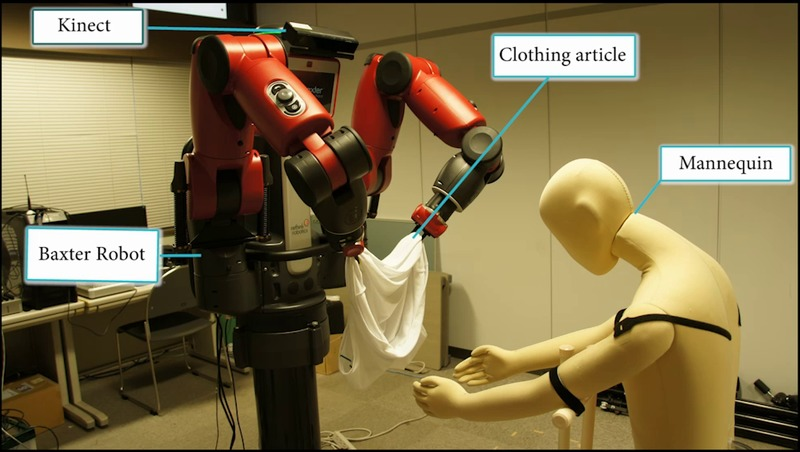
\includegraphics[width=\linewidth]{setup}
	\caption{Setup of robotic cloth manipulation task}
	\label{fig:setup}
\end{figure}

\section{Introduction}
\label{sec:introduction}
Due to the demographic trend in developed countries, robotic assistance in the field of elderly care in home environment is growing \cite{broekens2009assistive}. Although there has been a significant number of research done in this field, robotic clothing assistance is yet an open field for research. It is one of the basic and essential assistance activities in daily life of elderly as well as disabled people. While rigid object manipulation with robots has mainly relied on precise robot control, deformable objects rather require complex control scheme. Clothing assistance is a challenging problem since robot is required to manage two difficulties: (a) robot must do cooperative manipulation by holding cloth using both the arms while interacting with non-rigid and highly deformable cloth and (b) maintain safe human-robot interaction with the assisted person whose posture can vary during assistance.

In this study, we are investigating the applicability of using Dynamic Movement Primitives (DMP) as a task parameterization model for performing clothing assistance task. Robotic cloth manipulation task deals with putting a clothing article on both the arms. The idea of using DMP is inspired by the fact that DMP can learn complex task from the demonstration \cite{ijspeert2003learning, schaal2006dynamic, ijspeert2013dynamical} and thus reduce the manual efforts to design a controller from scratch or to fine-tune various controller parameters. We choose dual arm Baxter robot in this research as it is safe and flexible by design \cite{fitzgerald2013developing}.

Rest of the paper is organized as follows. Section \ref{sec:related_works}, gives brief overview of related literature in this field. In Section \ref{sec:method}, we introduce mathematical formulation about DMP followed by describing proposed method and its workflow. Section \ref{sec:experiments} deals with details of various experiments performed and their results. The discussion about experiments is presented in section \ref{sec:discussion}. Finally we conclude in section \ref{sec:conclusions} with some future directions.

\section{Related Works}
\label{sec:related_works}
There has been significant research done in the field of robotic clothing assistance by using vision system. Klee et al. \cite{klee2015personalized} worked on personalized assistance for dressing a user. The robot request user to move towards robot, monitors motion using vision module and puts a hat on user once users is reachable by the robot. They haven't considered human and cloth interaction. Yamazaki et al. \cite{yamazaki2013method, yamazaki2014bottom}  worked on bottom dressing by a life-sized humanoid robot, where they recognize the cloth state by using optical flow on the images acquired from a single camera. They did not handle large occlusions. Yamakawa et al. \cite{yamakawa2011dynamic} proposed a new strategy for dynamic manipulation of sheet-like flexible objects by a high-speed robot system. The proposed system learns necessary motor skills from demonstration performed by a human subject. They worked on fast cloth state tracking but it is not related to robotic clothing assistance.

Robotic cloth handling is challenging. Unlike rigid object manipulation using robots, which has mainly relied on precise robot control, deformable objects rather require complex control scheme. Many researchers have used vision information with combination of techniques such as motor skills learning using Reinforcement Learning. Colom{\'e} et al. \cite{colome2015friction} proposed a framework for Reinforcement Learning of robotic tasks in non-rigid environments by incorporating friction based model. Gao et al. \cite{gao2015user, gao2016iterative} have focused on user upper-body modeling for personalized dressing by using top-view depth camera with the help of randomized decision forests to estimate user pose. They proposed an online iterative path optimization method to enable Baxter robot to assist human in wearing a sleeveless jacket. Another interesting work by Kapusta et al. \cite{kapusta2016data} is focused towards designing a controller inspired from data-driven haptic perception. They classified the forces measured at robot's end effector by using hidden Markov models and performed clothing task using hospital gown. Their focus was to classify force data for haptic perception with high accuracy. Koganti et al. \cite{koganti2015cloth} proposed a framework for offline learning of cloth dynamics model using Gaussian Process Latent Variable Models (GP-LVM) by incorporating motion capture data and applying this model for online tracking of human-cloth relationship using a depth sensor. They showed that shared GP-LVM is able to learn reliable motion models of the T-shirt state for clothing task. Representing cloth state in low-dimensional field by using topology coordinates is another impressive work by Tamei et al. \cite{tamei2011reinforcement}. They proposed Reinforcement Learning framework and demonstrated that robot quickly learns a suitable arm motion for putting T-shirt into the mannequin's head. Another exciting work was done by Mons{\'o} et al. \cite{monso2012pomdp}, where they proposed a probabilistic planner, based on Partially Observable Markov Decision Process (POMDP) approach, for reducing the inherent uncertainty of cloth sorting (isolation/extraction) task. Their approach relaxes the precision requirements of robot vision and manipulation.

The problem of robotic clothing assistance not only depends on tracking cloth dynamics but also motor skills required to perform the task. A combination of such techniques is encouraged. However, we see that there has been a large gap when compared to the practical use cases in elderly care. The most important point should be learning rate of the task. We believe that \textit{Learning from Demonstration} frameworks are quick to learn in cases which involve complex task specific dynamics. The problem of putting sleeveless T-shirt into the arms of mannequin is close to the practical use case. Therefore, we are putting our efforts to solve it.

\begin{figure}
	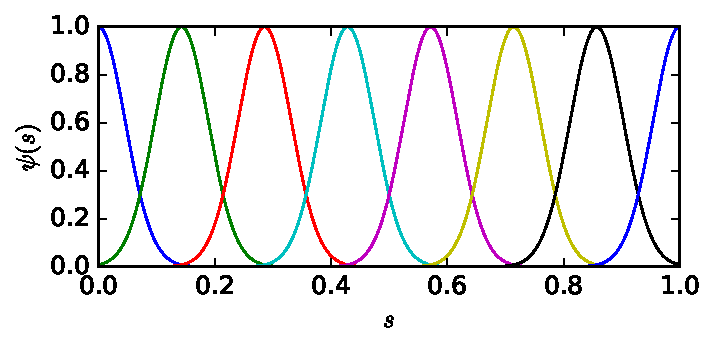
\includegraphics[width=\linewidth]{gaussian_kernels}
	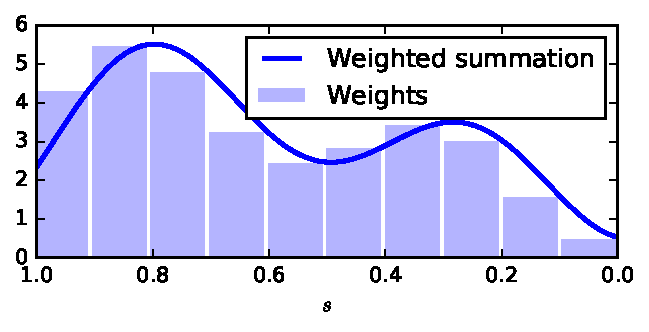
\includegraphics[width=\linewidth]{weighted_summation}
	\caption{$\psi(s)$ activations and weighted summation of Gaussians}
	\label{fig:psi_activations}
\end{figure}

\begin{figure*}
	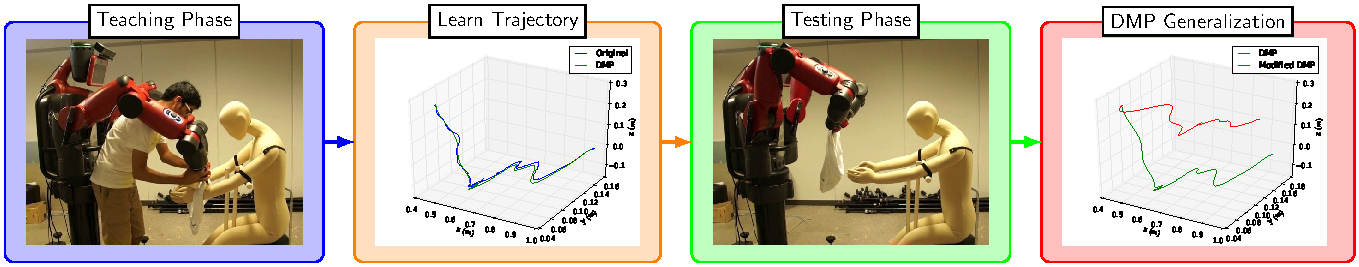
\includegraphics[width=\linewidth]{flowchart_conf}
	\caption{Workflow of robotic cloth manipulation task. Initially, a kinesthetic demonstration is performed with the robot controlled in gravity compensation mode. This demonstration is recorded and parameterized by DMP. Later on, posture of the mannequin is changed and accordingly start and goal parameter of DMP is modified. Now, modified DMP can accommodate new posture.}
	\label{fig:workflow}
\end{figure*}

\section{Method}
\label{sec:method}
Robotic cloth manipulation task deals with putting a clothing article on both the arms. We are using DMP framework to learn this complex task from demonstration and thus reduce the manual efforts to design the controller from scratch. We choose dual arm Baxter robot in this research. Following subsections explain about underlying DMP framework followed by the proposed method.

\subsection{Dynamic Movement Primitives}
\label{sec:dmp}
Dynamic Movement Primitives (DMP) aims at designing controller for learning and generalization of motor skills by learning from demonstration \cite{ijspeert2003learning}. The controller is based on nonlinear dynamical system and use locally weighted regression techniques to learn complex, discrete or rhythmic, movements demonstrated by a human subject \cite{ijspeert2002movement}. The controller can be considered to be discrete or rhythmic pattern generator which can replay and modulate the learned movements, while being robust against perturbations.

The basic idea behind DMP formulation is to use an analytically well-understood dynamical system and add a nonlinear term, so that it produces the desired behavior \cite{ijspeert2013dynamical}. Formally, it is defined by a damped spring model as below:

\begin{equation}
	\tau	 \dot{v} = K (g - x) -D v - K (g - x_0) s + K f(s)
\end{equation}
\begin{equation}
	\tau	 \dot{x} = v
\end{equation}

The term $x$ and $v$ are position and velocity of the system respectively, $x_0$ and $g$ are start and goal position, $\tau$ is a scaling term, $K$ is spring constant and $D$ is damping factor. The nonlinear function $f$, which is also called as forcing term is a non-linear function to be learned to allow complex movements. The forcing function $f$ is chosen as

\begin{equation}
	f(s) = \frac{\Sigma_{i} w_i \psi_i(s)}{\Sigma_{i} \psi_i(s)} s
	\label{eq:forcing_func}
\end{equation}

where $\psi_i$ is defined as Gaussian basis function as
\begin{equation}
	\psi_i = \textrm{exp}\left( -h_i \left( s - c_i\right)^2 \right)
\end{equation}

where $h_i$ and $c_i$ are constants that determine, respectively, width and centers of basis functions. $w_i$ represents weight defined for each Gaussian. Forcing function $f$ depends on phase variable $s$. Phase variable $s$ starts from $1$ and monotonically decreases to $0$, defined by equation below:

\begin{equation}
	\tau \dot{s} = - \alpha s
\end{equation}

where $\alpha$ is a positive gain term. Our goal is to design a forcing function that can learn from demonstration and allows us to scale the movement defined by goal state $g$. In other words, we want to setup a system which can follow specified path. The forcing term can be redefined as:

\begin{equation}
	f_{target}(s) = \frac{D v + \tau \dot{v}}{K} - - (g - x) +  (g - x_0) s
\end{equation}

where desired acceleration $\dot{v}(t)$ can be calculated by double differentiating position data recorded from demonstration as

\begin{equation}
	\dot{v}(t) = \frac{\partial}{\partial t} v(t) = \frac{\partial}{\partial t} \frac{\partial}{\partial t} x(t)
\end{equation}

The forcing function [\ref{eq:forcing_func}] is comprised of weighted summation of Gaussian that are going to be activated as system converges to goal as shown in figure \ref{fig:psi_activations}. We want that forcing function matches the desired trajectory. In other words, we want $f_{target}$ to be as close as possible of $f$ as written below:

\begin{equation}
	J = \sum_{s} \left( f_{target}(s) - f(s) \right)^2
\end{equation}

This ends by calculating weight parameters across Gaussians. Optimization methods such as locally weighted regression \cite{vijayakumar2000locally} can be used, so that forcing function matches desired trajectory. This way DMP can be made to imitate desired path \cite{pastor2009learning}.

\subsection{Robotic cloth manipulation using DMP}
\label{sec:system_overview}
In this section, we provide brief overview of our system. As per the formulation described in section \ref{sec:dmp}, DMP can learn from demonstration. Therefore we start by performing a kinesthetic demonstration with the robot controlled in gravity compensation mode as shown in figure \ref{fig:workflow}. This is referred as ``Teaching Phase'', since in this phase, we are teaching skills to robot to perform the task.  During the demonstration, pose trajectory of end-effector is recorded using Baxter API and stored in a file. The term pose collectively refers to position as cartesian position $p = (p_x, p_y, p_z) \in \mathbb{R}^3$ and orientation as quaternion $q = (q_x, q_y, q_z, q_w) \in \mathbb{R}^4$. Once the demonstration is finished, DMP is parameterized using recorded trajectory file. This is termed as ``Learn Trajectory'' phase. The parameterized DMP can represent all the characteristics of original trajectory. Here, three DMP systems, one for each coordinate axis i.e., $x$, $y$ and $z$ are initialized for one arm. In this way, we have total six DMP systems, which can control both the arms of Baxter robot. In ``Testing Phase'', we change the posture of mannequin by changing the angle of inclination as shown in figure \ref{fig:inclination}. At this point, we use Kinect Sensor to get the 3D coordinates of wrist and shoulder of mannequin. We change start and goal parameter of DMP trajectories by using this information. In this way, we have generalized DMP system, which can adapt modified posture referred as ``DMP Generalization''. Before using Kinect Sensor, it is extremely important to do Kinect-Baxter calibration, so that 3D coordinates are translated from Kinect space to Baxter space. For Kinect-Baxter calibration, we collect a dataset of points observed by Baxter and Kinect. Then we use absolute orientation calibration \citep{umeyama1991least} to align the frames of reference.

We have divided the complete trajectory into two parts: (a) The reaching part, which refers to the trajectory starts from home position of robot and ends till hands of mannequin (b) the clothing part, which refers to the trajectory starts from hands of mannequin and reaches upto shoulder nearly. The reaching part can be performed through simple position based controller but for the clothing phase, we need to train DMP since this part changes drastically between postures and can be prone to failure.

\begin{figure}
	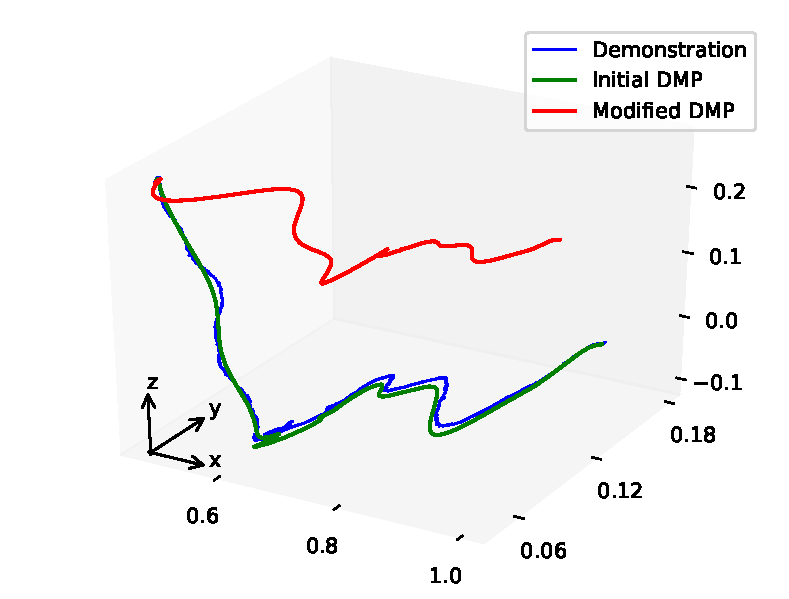
\includegraphics[width=\linewidth]{all_traj}
	\caption{Left arm trajectory of Baxter}
	\label{fig:trajectory}
\end{figure}

\section{Experiments}
\label{sec:experiments}
Robotic cloth manipulation task contains a dual arm humanoid robot Baxter. Setup of our system is shown in figure \ref{fig:setup}. We choose soft mannequin instead of a human for this experiment. Both the arms of mannequin are open and given support by a metallic stand, to avoid falling down the arms. Mannequin is positioned in such a way so that it resides within limits of workspace of Baxter robot. Both the arms of mannequin are facing towards robot. A Kinect V2 \cite{microsoft2014kinect} sensor is mounted on LCD display of Baxter robot. Kinect sensor can see the mannequin and clothing article and provides depth information, which is necessary for mannequin tracking. The clothing article is put in the arms of Baxter robot manually before starting experiment.

Baxter robot is connected to a computer directly using Ethernet cable. It is controlled using Robot Operating System (ROS) \cite{quigley2009ros}, one of the widely used tools by the researchers in robotics community. We used Baxter robot's API, which is available and supported by ROS to command the robot. Kinect sensor is controlled by open source Kinect API for ROS \cite{iai_kinect2, libfreenect2}. We performed following two experiments to validate our approach: (a) Clothing task using position DMP (b) Failure detection using end-effector forces.

\subsection{Clothing task using position DMP}
The aim of this experiment is to put sleeveless T-shirt on both the arms of mannequin by using DMP system. We use position data to initialize DMP trajectories, which are being used in this task. The posture of mannequin is changed. At this point, we use Kinect Sensor to get 3D coordinates of wrist and shoulder of mannequin. Now we change start and goal parameter of DMP trajectories by using this information. Modified DMP can be acquired by rolling out DMP system as described in section \ref{sec:dmp}.

In this experiment, the initialized DMP was modified to accommodate new posture by changing start and goal parameter of DMP. The generated trajectory was then run on Baxter robot as shown in figure \ref{fig:trajectory}. Newly generated DMP trajectory (shown in red color) was not only found well suited and capable of performing clothing task but also smooth compared to original trajectory (shown in blue color). A video demonstration of this experiment can be seen at YouTube\footnote{\url{http://youtu.be/Rb2JePazJjk}}.

To evaluate this experiment, we performed it many times and monitored trajectory generated by DMP system. We defined angle of inclination as the angle between arm of mannequin and horizontal axis.  The angle of inclination is defined in clockwise direction, hence it is $+ve$ when arms are inclined upward, similarly it is $-ve$ when arms are inclined downward. It was changed by keeping arms at different-different height. The accuracy measurement is shown in figure \ref{fig:accuracy}. It was observed that DMP system was able to generate the appropriate trajectory for a range of $20^\circ$ and it never failed in this range. However, as we keep on going far away from the original posture, success rate starts declining and finally reached to $0$. 

\begin{figure}
	\centering
	\begin{subfigure}{.5\linewidth}
		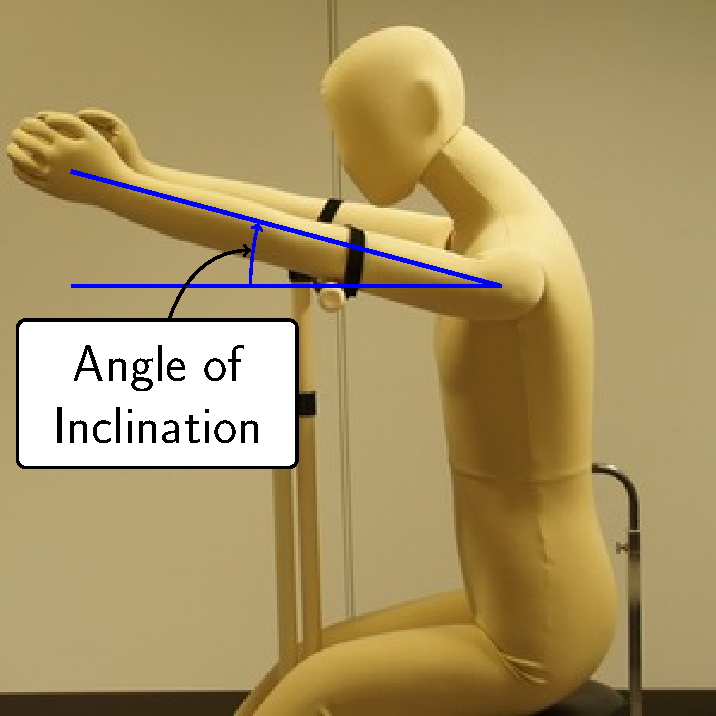
\includegraphics[width=.9\linewidth]{inclination_plus}
	    \caption{Positive angle}
	\end{subfigure}%
	\begin{subfigure}{.5\linewidth}
		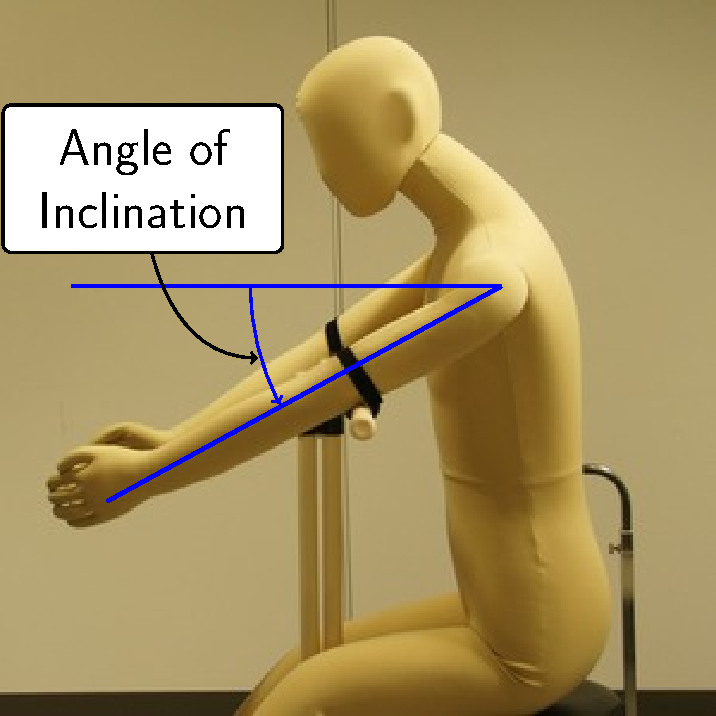
\includegraphics[width=.9\linewidth]{inclination_minus}
	    \caption{Negative angle}
	\end{subfigure}
	\caption{Angle of Inclination}
	\label{fig:inclination}
\end{figure}

\begin{figure}
	\centering
	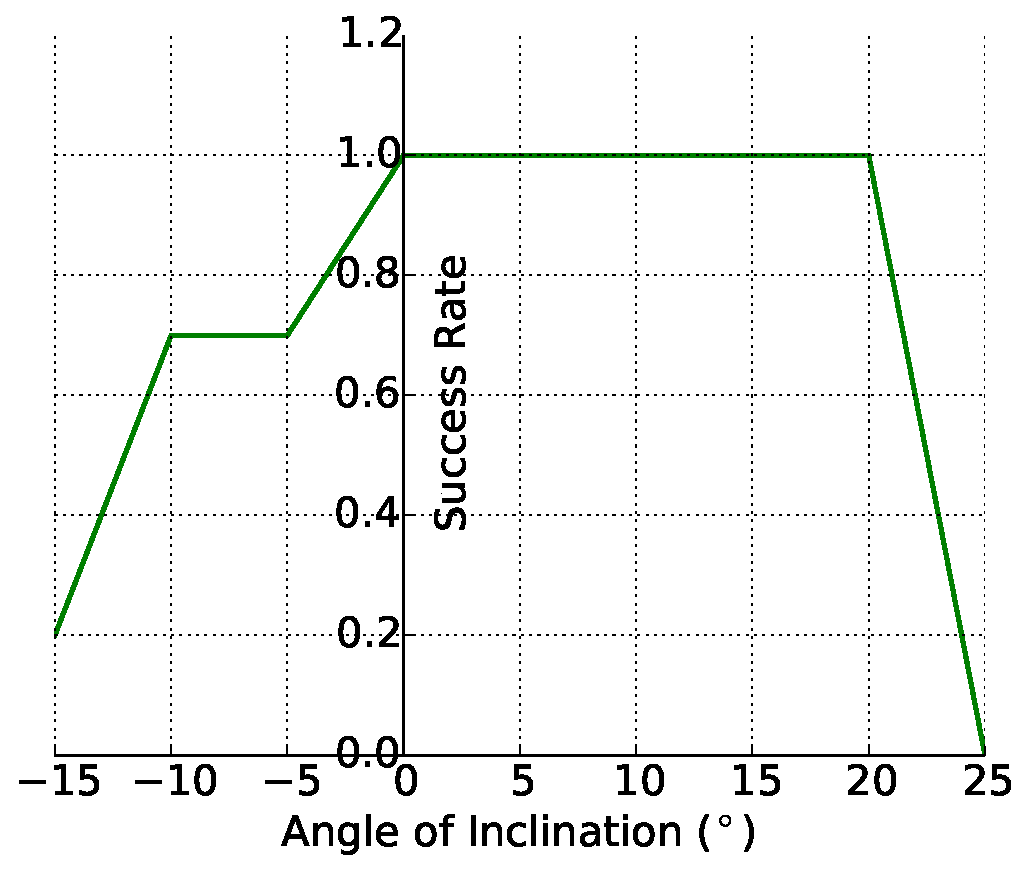
\includegraphics[width=\linewidth]{success_rate}
	\caption{Accuracy measurement}
	\label{fig:accuracy}
\end{figure}

\subsection{Failure detection using end-effector forces}
This experiment is designed to deal with failure cases. There can be many failure cases during the task, such as clothing article gets stuck into the fingers, sleeve getting stuck on the arms, sleeve not entering the arm but entirely missing etc, as shown in figure \ref{fig:failure_scenarios}. In this experiment, we are using forces being applied on the end-effector of Baxter robot to detect failure scenario. Appropriate action can be taken once the failure is detected.

The clothing task has to deal with complex dynamics including manipulation of clothing article. Clothes are non-rigid, flexible and highly deformable objects, making the task more difficult to perform. During the task, we observed forces being applied at both the end-effector of Baxter robot. Trajectories were monitored and categorized into two \textit{success} and \textit{failure}. The mean of these two categories is calculated and plotted as shown in figure \ref{fig:position_force}. Force value is the norm of force applied in all three cartesian directions. This is the average profile over several \textit{success} and \textit{failure} trajectories for different postures of left arm of mannequin. 

It is clearly visible from the figure \ref{fig:position_force} that the applied forces are very different in nature in both the cases. Both of these forces are increasing from the beginning, however, forces in case of \textit{failure} are much higher than that of \textit{success}. Hence one can easily differentiate and detect the failure by using this information.

\begin{figure}
	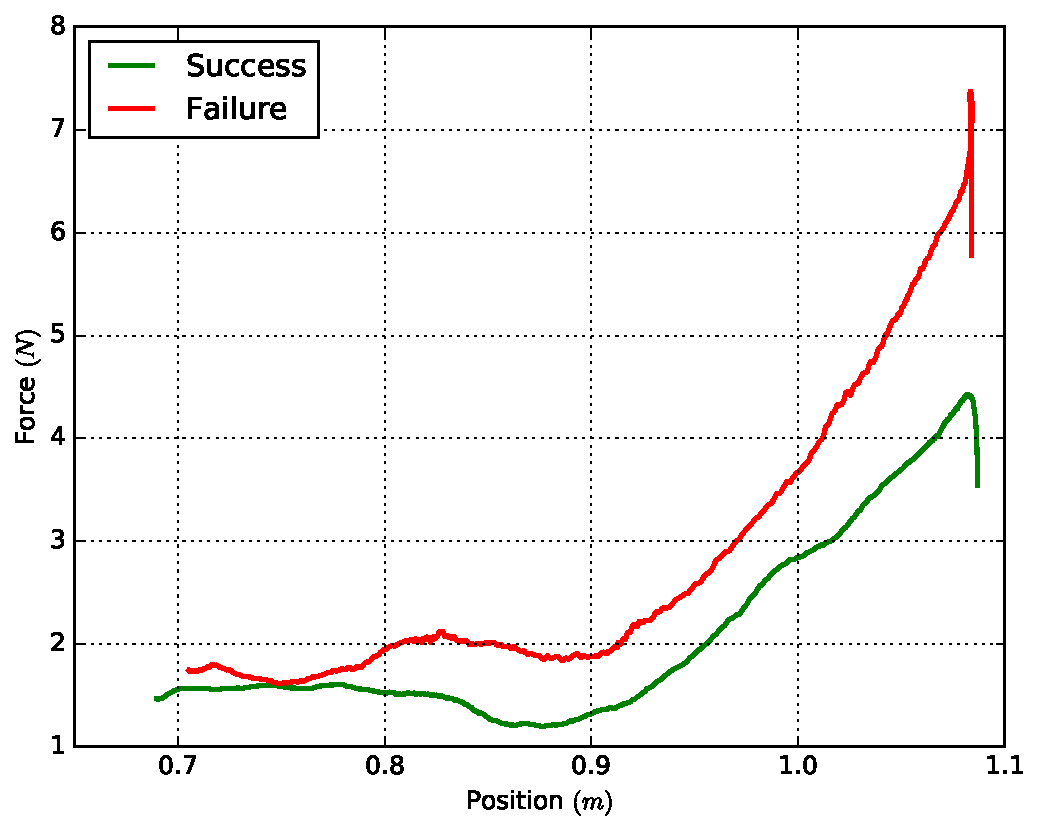
\includegraphics[width=.9\linewidth]{position_force}
	\caption{Failure detection using end-effector forces}
	\label{fig:position_force}
\end{figure}

\begin{figure}
	\centering
	\begin{subfigure}{.4\linewidth}
		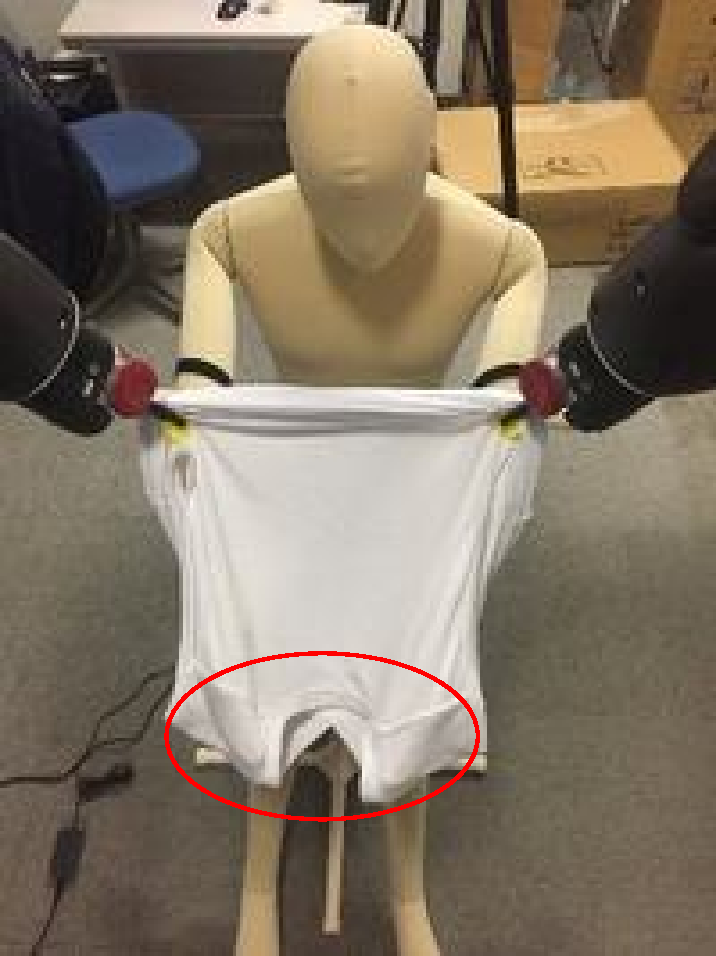
\includegraphics[width=.98\linewidth]{failure_scenario_1}
	\end{subfigure}%
	\begin{subfigure}{.4\linewidth}
		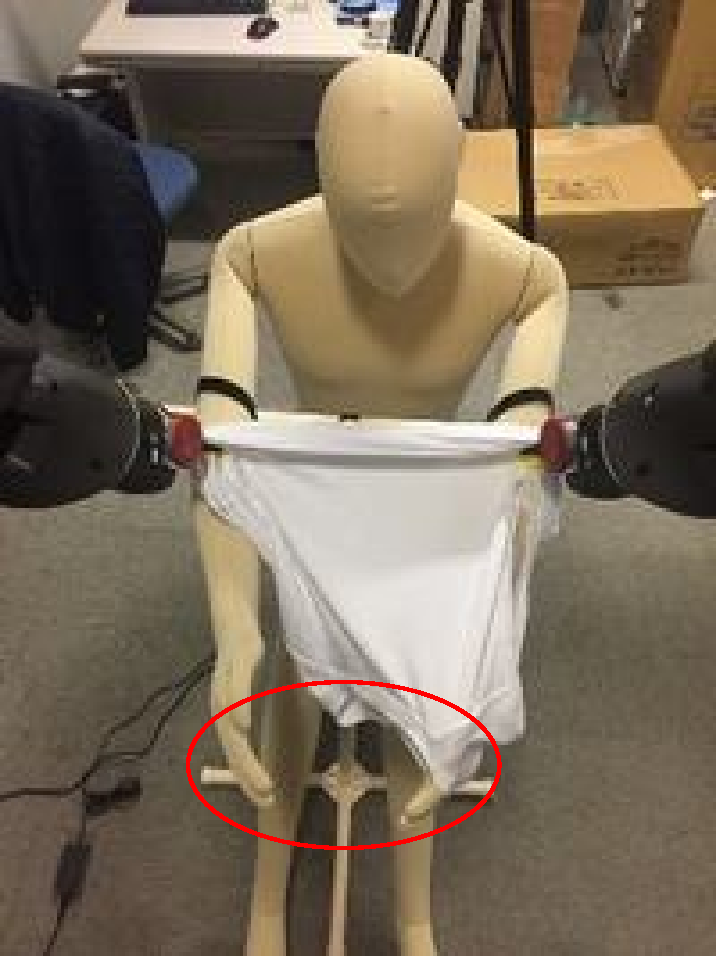
\includegraphics[width=.98\linewidth]{failure_scenario_2}
	\end{subfigure}
	\begin{subfigure}{.4\linewidth}
		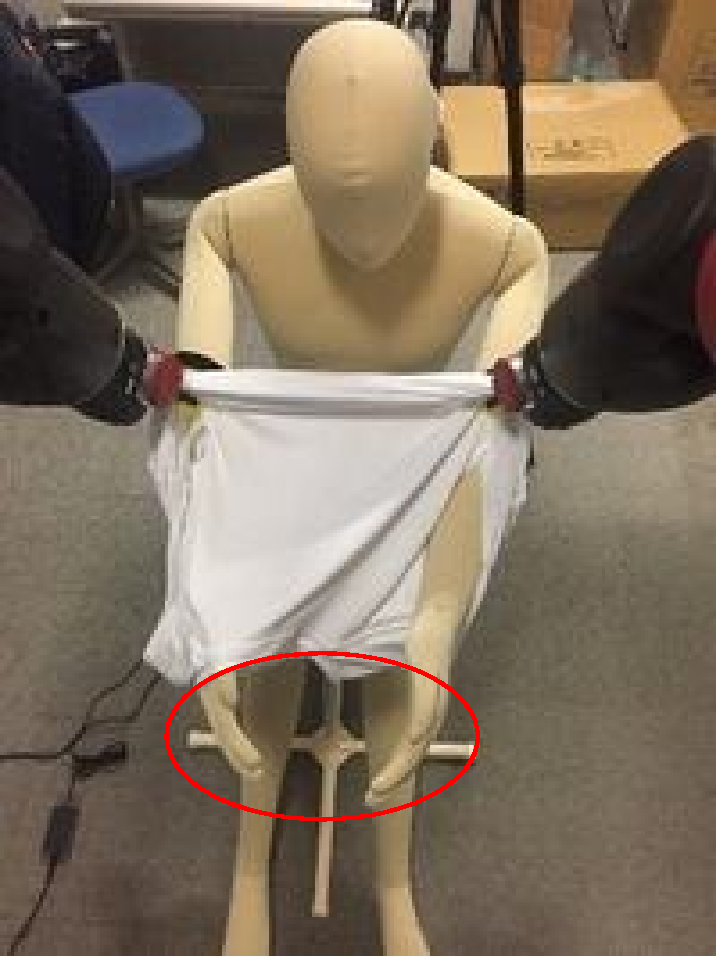
\includegraphics[width=.98\linewidth]{failure_scenario_3}
	\end{subfigure}%
	\begin{subfigure}{.4\linewidth}
		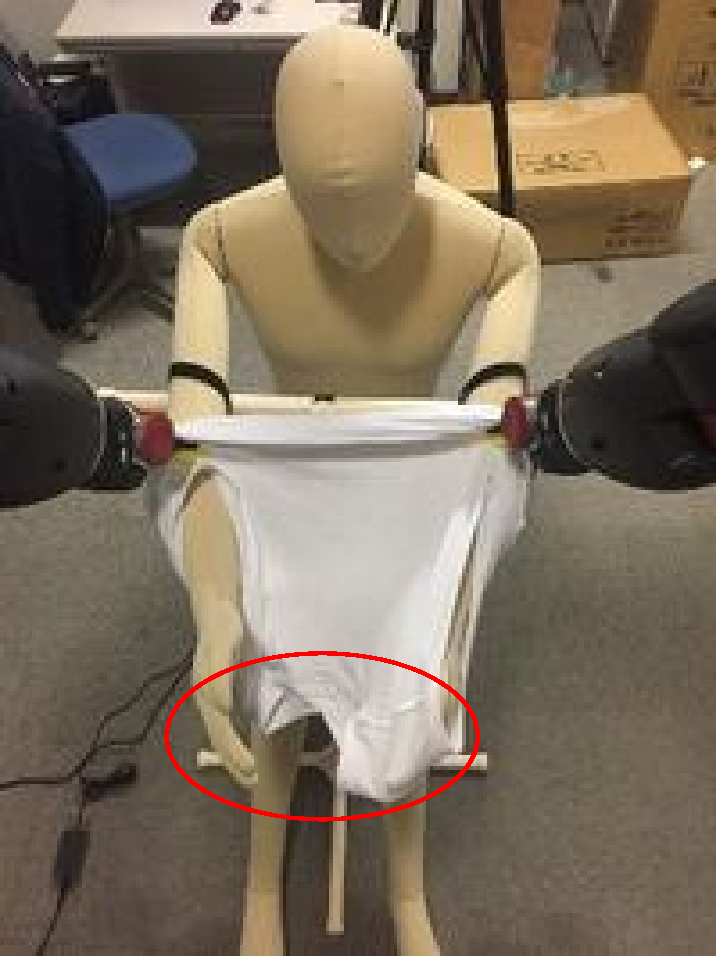
\includegraphics[width=.98\linewidth]{failure_scenario_4}
	\end{subfigure}
	\caption{Various Failure Scenarios}
	\label{fig:failure_scenarios}
\end{figure}

\section{Discussion}
\label{sec:discussion}
The clothing assistance task deals with manipulation of highly deformable clothing article, which inherits complex dynamics. Failure can be detected by observing end-effector forces. The shape of clothing article keeps on changing during each trail, which affects the task settings. That is why, a trajectory which was able to preform successfully in the past, doesn't work later sometimes. We noticed that there can be many failure scenarios such as clothing article gets stuck into the fingers, sleeve getting stuck on the arms, sleeve not entering the arm but entirely missing etc. Proposed failure detection method by using force information can detect failures when clothing article is stuck tightly. The other reason of failure can be position based DMP system. Orientation plays a major role in the task however DMP system was initialized by position data while ignoring the orientation of end-effector. The orientation was kept same as it was in original trajectory. 

\section{Conclusions}
\label{sec:conclusions}
This paper presents an approach for robotic cloth manipulation for clothing assistance task using Dynamic Movement Primitives. A dual arm Baxter robot, soft mannequin, and very thin sleeveless T-shirt were used in the task. We have also presented an approach for failure detection using forces being applied on end-effector of the robot. We have used the Baxter APIs in order to get the forces, which are calculated by Baxter Dynamics Module. Though raw forces were very noisy in nature, but after applying median filter most of the noise was eliminated properly.

We plan to extend our research to make the approach more robust by adding visual information and force information with DMP system in near future. Also, there is a need for designing an adaptive controller for real-time tracking to adapt and detect various failure scenarios. DMP system also needs to be improved to incorporate orientation information of end-effector. Therefore, in the future, a combination of robot vision and force data can provide better estimation of cloth state.

\begin{acks}
	The authors would also like to thank the anonymous referees for their valuable comments and helpful suggestions. The work is supported by the \grantsponsor{GS501100001809}{National Natural Science Foundation of China}{http://dx.doi.org/10.13039/501100001809} under Grant No.:~\grantnum{GS501100001809}{61273304} and~\grantnum[http://www.nnsf.cn/youngscientsts]{GS501100001809}{Young Scientsts' Support Program}.
\end{acks}

\bibliographystyle{ACM-Reference-Format}
%\bibliographystyle{unsrt}
\bibliography{air}

\end{document}
